
\begin{definition}{Sekanten-Steigung und Differentialquotient}\\
    Sei $f$ eine Funktion und $\left[x_{0}, x_{0}+h\right]$ ein Intervall im Definitionsbereich von $f$. Der Quotient
    
    $$\frac{\Delta f}{\Delta \mathrm{x}}=\frac{f\left(x_{0}+h\right)-f\left(x_{0}\right)}{h}$$
    
    heisst Differentialquotient von $f$.
\end{definition}

\begin{center}
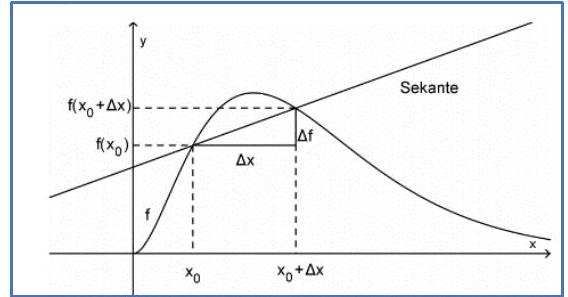
\includegraphics[scale=0.3]{Analysis1/zsf/Images/Differential/2024_01_20_7bfda6c084929ccc01ffg-03.jpg}
\end{center}

\begin{definition}{Differenzierbarkeit}\\
    $f$ ist in $x_0$ \emph{differenzierbar}, falls der Grenzwert $\lim_{x \to x_0} \frac{f(x) -f(x_0)}{x -x_0}$
    existiert.\\
    Ist dies der Fall, wird der Grenzwert mit $f'(x)$ bezeichnet.
        $$
        f'(x_0) = \lim_{h \to 0}\frac{\Delta f}{\Delta \mathrm{x}} = \lim_{h \to 0}\frac{f(x_0 + h) -f (x_0)}{h}
        $$
    Den Grenzwert selbst bezeichnet man als Ableitung.
    \tcblower 
    Vereinfacht: Eine Funktion ist differenzierbar, falls die Kurve keine Knicke macht.
\end{definition}

\begin{formula}{Tangentengleichung}
    $$
    y=f^{\prime}\left(x_{0}\right) \cdot\left(x-x_{0}\right)+f\left(x_{0}\right)
    $$
\end{formula}

\begin{definition}{Stetige Differenzierbarkeit}
	Eine Funktion ist stetig differenzierbar, wenn sie differenzierbar ist und ihre Ableitungsfunktion stetig ist.
\end{definition}






